\documentclass[12pt, %
openright, 
oneside, %
%twoside, %TCC: Se seu texto tem mais de 100 páginas, descomente esta linha e comente a anterior
a4paper,    %
%english,   %
brazil]{facom-ufu-abntex2}

\usepackage{graphicx}
\graphicspath{{figuras/}{pictures/}{images/}{./}} % where to search for the images

\newcommand{\blue}[1]{\textcolor{blue}{#1}}
\newcommand{\red}[1]{\textcolor{red}{#1}}


\autor{Pedro Henrique Bufulin de Almeida} %TCC
\data{2021}
\orientador{Pedro Frosi Rosa} %TCC
%\coorientador{Algum?} %TCC

% ---
% Informações de dados para CAPA e FOLHA DE ROSTO
% ---
 
\titulo{Sistema de segurança doméstica: uma solução open source e com privacidade} %TCC

\hypersetup{pdfkeywords={palavra 1}{palavra 2}{palavra 4}{palavra 4}{palavra 5}} %TCC

\begin{document} 
\frenchspacing 

% ----------------------------------------------------------
% ELEMENTOS PRÉ-TEXTUAIS
% ----------------------------------------------------------
%\pretextual
\imprimircapa
\imprimirfolhaderosto


% ---
% Inserir folha de aprovação
% ---
%
% \includepdf{folhadeaprovacao_final.pdf} %TCC: depois de aprovado o trabalho, descomente esta linha e comente o próximo bloco para incluir scan da folha de aprovação.
%
\begin{folhadeaprovacao}

  \begin{center}
    {\ABNTEXchapterfont\large\imprimirautor}

    \vspace*{\fill}\vspace*{\fill}
    {\ABNTEXchapterfont\bfseries\Large\imprimirtitulo}
    \vspace*{\fill}
    
    \hspace{.45\textwidth}
    \begin{minipage}{.5\textwidth}
        \imprimirpreambulo
    \end{minipage}%
    \vspace*{\fill}
   \end{center}
    
   Trabalho aprovado. \imprimirlocal, 01 de novembro de 2016: %TCC:

   \assinatura{\textbf{\imprimirorientador} \\ Orientador}  
   \assinatura{\textbf{Professor}}% \\ Convidado 1} %TCC:
   \assinatura{\textbf{Professor}}% \\ Convidado 2} %TCC:
   %\assinatura{\textbf{Professor} \\ Convidado 3}
   %\assinatura{\textbf{Professor} \\ Convidado 4}
      
   \begin{center}
    \vspace*{0.5cm}
    {\large\imprimirlocal}
    \par
    {\large\imprimirdata}
    \vspace*{1cm}
  \end{center}
  
\end{folhadeaprovacao}
% ---


%%As seções dedicatória, agradecimento e epígrafe não são obrigatórias.
%%Só as mantenha se achar pertinente.

% ---
% Dedicatória
% ---
%\begin{dedicatoria}
%   \vspace*{\fill}
%   \centering
%   \noindent
%   \textit{Dedico a \lipsum[10]}  %TCC:
%   \vspace*{\fill}
%\end{dedicatoria}
% ---

% ---
% Agradecimentos
% ---
%\begin{agradecimentos}
%Agradeço a \lipsum[30]. %TCC:
%\end{agradecimentos}
% ---

% ---
% Epígrafe
% ---
%\begin{epigrafe}
%    \vspace*{\fill}
%	\begin{flushright}
%		\textit{``Alguma citação que ache conveniente? \lipsum[10]''} %TCC:
%	\end{flushright}
%\end{epigrafe}
% ---



\begin{resumo} %TCC:
 Os sistemas de segurança domésticos carecem de soluções
 que sejam customizáveis de acordo com a falha de segurança que existe em cada domicílio.
 Frequentemente encontra-se no mercado câmeras que fazem apenas a gravação com baixa resolução, e
 caso busque algo mais sofisticado, existem modelos envolvendo reconhecimento facial, mas eles são ainda mais caros e raros.
 Além disso, as soluções de segurança pública ou providas por empresas privadas, quando existem, podem usar as informações 
 coletadas para seus próprios benefícios, diminuindo a privacidade do indivíduo. Este trabalho propõe uma solução que seja
 fácil de implementar, com ferramentas prontas para uso e customizável por ser de código aberto,  
 trazendo com esta última característica o poder para qualquer um de criar a sua própria segurança 
 e modificar este projeto de acordo com suas necessidades. 

 \vspace{\onelineskip}
    
 \noindent
 \textbf{Palavras-chave}: Segurança, código,  aberto, reconhecimento, facial, câmera.  %TCC:
\end{resumo}

% ---
% inserir lista de ilustrações
% ---
\pdfbookmark[0]{\listfigurename}{lof}
\listoffigures*
\cleardoublepage
% ---

% ---
% inserir lista de tabelas
% ---
\pdfbookmark[0]{\listtablename}{lot}
\listoftables*
\cleardoublepage
% ---



% ---
% inserir lista de abreviaturas e siglas
% ---
\begin{siglas} %TCC: 
  \item[API] Application Programming Interface
  \item[REST] Representational State Transfer
  \item[HSL] HTTP Live Streaming
  \item[RTMP] Real Time Messaging Protocol 
  \item[LBPH] Local Binary Patterns Histogram 
\end{siglas}
% ---

%% ---
%% inserir lista de símbolos, se for adequado ao trabalho. %TCC:
%% ---
%\begin{simbolos}
%  \item[$ \Gamma $] Letra grega Gama
%  \item[$ \Lambda $] Lambda
%  \item[$ \zeta $] Letra grega minúscula zeta
%  \item[$ \in $] Pertence
%\end{simbolos}
%% ---

% ---
% inserir o sumario
% ---
\pdfbookmark[0]{\contentsname}{toc}
\tableofcontents*
\cleardoublepage
% ---





% ----------------------------------------------------------
% ELEMENTOS TEXTUAIS
% ----------------------------------------------------------
\textual


% ----------------------------------------------------------
% Introdução
% ----------------------------------------------------------

\chapter[Introdução]{Introdução}
%TCC:
% Contextualização, problema, hipótese, objetivo geral, objetivos específicos, justificativa e resultados esperados.
Em 2019 foi estimado que existem 200 milhões de câmeras de vigilância na China e na última década,
avanços tecnológicos tornaram essas câmeras ainda mais eficientes em monitorar 1.4 bilhões de chineses. 
Ainda segundo o autor, o reconhecimento de rostos por câmeras começou a ser uma realidade em 2010 quando pesquisadores 
descobriram algoritmos de deep learning usados para reconhecer imagens e voz. Esses algoritmos podem
também inferir em tempo real a quantidade e a densidade de pessoas numa dada imagem
\cite{qiang2019road}. É notável que esse nível de vigilância está se tornando uma realidade em muitos outros
países no mundo além da China. Nesse sentido, é perceptível que existe uma demanda por aumentar a segurança usando os meios 
necessários, mas sem que isso signifique diminuir a privacidade dos indivíduos colocando suas informações disponíveis aos 
governantes e corporações.

Em questão de proteção da privacidade, tecnologias de código aberto podem oferecer uma solução. Quando o Desenvolvimento
ocorre em aberto, é possível verificar diretamente se o proprietário está ativamente buscando segurança e privacidade e
entender como ele trata esses problemas. A possibilidade de estudar o processo seguido faz com que qualquer um possa
realizar uma auditoria independente. \cite{mardjan2016open}

Considerando-se a necessidade de criar uma solução que traga os benefícios da vigilância e mantendo a privacidade individual, surge
essa proposta da construção de um sistema de segurança doméstica que oferece as opções de reconhecimento de imagem
por inteligência artificial, além da visualização em tempo real da gravação, e que tenha tanto o código fonte quanto o hardware
abertos em virtude da transparência.

\section{Objetivos}

O objetivo principal deste trabalho é performar a concepção, modelagem e implementação de um sistema de segurança doméstica utilizando
apenas hardware e software que sejam abertos, assim como o projeto resultante final deverá ser. Pretende-se que seja possível visualizar 
a imagem da câmera em tempo real, adicionar rostos de pessoas que sejam tidos como confiáveis e não passíveis de alarme, enviar notificações
para o usuário quando for identificado alguém na câmera que não passar como confiável. Também será disponibilizada uma documentação que 
contém as instruções para implementar o sistema em domicílio, para que qualquer indivíduo provido do equipamento possa colocá-lo em uso.

\section{Método}

Para os objetivos apresentados Seção 1.1 serem alcançados, os seguintes passos serão seguidos para o desenvolvimento deste sistema:

\begin{itemize}
    \item  Criar um protótipo de solução para a questão apresentada:
    \begin{itemize}
      \item Definir a arquitetura do sistema, tanto do backend quanto do frontend.
      \item Definir o tipo de API e qual a melhor linguagem para criá-la.
      \item definir qual o hardware a ser utilizado, tanto da câmera quanto do sistema que processará as informações da câmera. 
      \item Explorar as capacidades do hardware da câmera e do sistema que coordena suas ações, além de encontrar suas limitações e como contorná-las.
      \item Se for necessário, definir como implementar um servidor para que seja processada e armazenada a imagem da câmera.
  \end{itemize}
\end{itemize}

\begin{itemize}
  \item  Programar o protótipo que solucionará o problema apresentado:
  \begin{itemize}
    \item Escolher algoritmos de compressão de imagem adequado para as gravações.
    \item Implementar a aplicação de acesso do usuário.
    \item Implementar o software que será responsável pelo reconhecimento de imagem e streaming do vídeo para o aplicativo.
  \end{itemize}
\end{itemize}




\chapter{Fundamentação Teórica}


Neste capítulo estão as tecnologias e os conceitos que serão utilizados no decorrer da construção deste projeto.
São conceitos relacionados à arquitetura do sistema que será construído, as abordagens que já existem, \emph{hardware}, 
linguagens e \emph{frameworks} que serão utilizados.


\section{Arquitetura de transmissão em tempo real}
 
A figura abaixo mostra um sistema de cliente-servidor para trocar de dados de multimídia.
Na origem, tem-se a gravação comprimida, codificada e armazenada no dispositivo de armazenamento,
como um disco rígido, por exemplo. Em seguida, por meio de algum software de tratamento de mídia que será produzido,
esses arquivos são requisitados por usuários e entregues de acordo. Um protocolo de transferência é utilizado para
entregar os dados de multimídia para o cliente (tais como RTMP ou HLS), onde eles são primeiramente armazenados
na memória principal e eventualmente decodificados e apresentados ao usuário. \cite{lee2005scalable}


\begin{figure}[!ht]
  \centering
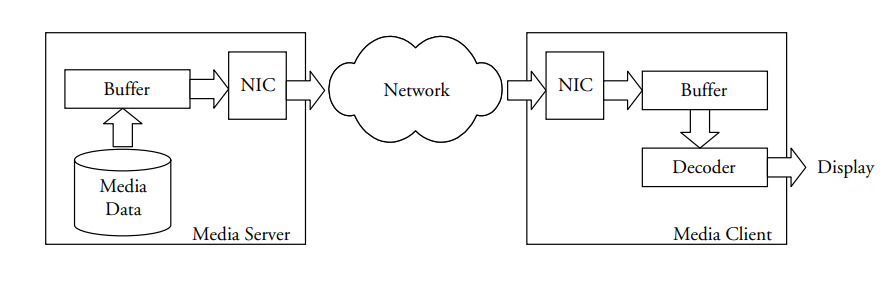
\includegraphics[width=1\linewidth]{Capturar.PNG}
\caption[Representação de um arquitetura de tempo real genérica]{Arquitetura genérica de transmissão em tempo real}
\label{fig:graficosVariandoTamanhoRede}
\end{figure}

Esta arquitetura é a que levarei em consideração na implementação do projeto. O servidor que será implementado utilizando
um microcomputador contem a câmera e sistema operacional para realizar o processamento e transmissão dos dados de 
multimídia. Outra alternativa seria o microcomputador apenas enviar os fluxo de vídeo para um terceiro servidor que faria o processamento
da imagem caso a capacidade daquele não seja suficiente, resultando em um sistema distribuído. Essa outra abordagem também
respeita a arquitetura citada acima.



\section{Framework de desenvolvimento front end}

Como é de se esperar, um sistema que permite a visualização em tempo real necessitará
de um meio para apresentar ao usuário as saídas e o resultado do processamento delas.
Como se trata de um sistema de segurança, o mais viavel é que o usuário sempre tenha 
em mãos o dispositivo que fornece a imagem, ou seja, o \emph{smartphone}. Portanto, faz sentido utilizar um \emph{framework}
que permita a criação de um front end mobile. Além disso, a aplicação resultante
deverá ser replicável em múltiplos dispositivos, para que o usuário não seja tolhido por não ter o meio adequado.
Dadas essas condições, o \emph{framework} que satisfaz elas é o \emph{React Native}

O React Native é um framework de desenvolvimento mobile híbrido (iOS e Android simultâneamente) voltado para a construção de interfaces
de usuário criado 
pelo facebook, utilizando \emph{javascript} com a linguagem de programação e compilando-o de forma que
seja executável pela plataforma nativa. Vale lembrar que o React Native não é 
uma solução \emph{full-stack} que vai lidar com tudo desde o banco de dados à atualizações em tempo real
de \emph{web sockets}. Ele é simplesmente a \emph{View layer} da aplicação. \cite{boduch2017react}


\section{Tecnologias de desenvolvimento back end}

O back end é a parte do sistema que realizará o processamento da imagem
que consiste de um servidor contendo o
banco de dados e uma aplicação que fornece os \emph{endpoints} responsáveis pela comunicação
com o front end. Nesses \emph{endpoints}, o usuário consegue fazer o envio, requisição e alteração
de dados por meio da abstração fornecida pelo front end. 

% Neste trabalho, o back end é responsável pelo processamento da imagem assim como pela criação do 
% canal de transmissão em tempo real dela. Além disso, existirá um \emph{endpoint} que permite
% o cadastro de um rosto específico, evitando que o sistema emita um alerta para essa pessoa.

Neste trabalho, a aplicação do \emph{back end} será feita utilizando o \emph{NodeJS}, que é um
ambiente de execução de javascript no servidor baseado em \emph{event-driven architecture} capaz
de entrada e saída assíncrona, muito utilizado em aplicações de comunicação em tempo real. \cite{aboutnodejs}
Além disso, Em Node.js, HTTP é um cidadão de primeira classe, projetado para que tenha um alta taxa de fluxo e baixa latência. 
Isso torna o Node.js uma ótima escolha para servir como base para uma biblioteca web ou para um framework. \cite{NodeJSaboutoriginal}.
Mais um motivo para a utilização de Node.js, é a grande quantidade de módulos disponíveis no npm. Este projeto particularmente
utilizará vários deles, sendo os principais o Express e o node-media-server. O primeiro facilita a criação da aplicação web no servidor,
e o segundo servirá para utilizar o protocolo RTMP, que é o ideal para transmissão de vídeo e áudio em alta performance. 
 
Também é necessária a implementação de um banco de dados que se comunicará com a aplicação do servidor. Para este projeto,
foi escolhido o PostgreSQL, sendo ele um banco de dados relacional de código aberto. Este sistema de banco de dados foi escolhido
por possuir \emph{Write-ahead Logging}, \emph{point-in-time-recovery}. Essas duas características são importantes para garantir
a confiabilidade e a possível recuperação dos dados em caso de perda. Além disso, a comunidade ativa do PostgreSQL é responsável
por criar diversas extensões e alguma delas podem ajudar no desenvolvimento do projeto. O último aspecto importante dessa escolha,
é que esse sistema de banco de dados também permite \emph{multi-factor authentication}. \cite{aboutPostgre}

Uma última camada de segurança da aplicação é necessária, de forma que tanto as informações do usuário
quanto o servidor em si estejam protegidos de possíveis ataques. Para proteger o servidor de acesso indevido aos \emph{endpoints}
vou utilizar o JSON Web Token (JWT). O JSON Web Token é um meio de representar reivindicações à serem transferidas entre duas partes.
Os dados são codificados com um JSON que é usado como o \emph{payload} de uma estrutura  JSON Web Encryption (JWE), permitindo que essas
reivindicações sejam assinadas digitalmente ou a integridade protegida com \emph{Message Authentication Code} ou criptografada. \cite{jsonwebtoken}

\section{Algoritmo de reconhecimento facial}

Para a funcionalidade de reconhecimento facial da câmera, usarei uma biblioteca de código aberto
de \emph{computer vision} chamada \emph{OpenCV}. Essa biblioteca possui mais de 2500 algoritmos
otimizados, incluindo os clássicos e os mais recentes do estado da arte. Eles podem ser utilizados
para detectar e reconhecer faces, identificar objetos classificar ações humanas em vídeo e mais. \cite{opencv}.
Ela suporta múltiplas linguagens incluindo Java, C++ e Python. para este trabalho, será usada a biblioteca em Python.

Para realizar o reconhecimento facial, é preciso conseguir antes reconhecer que há um rosto em vídeo.
O método que utilizarei, facilitado pelo \emph{OpenCV}, é o chamado \emph{Haar Cascades} \cite{viola2001rapid}.
Este algoritmo é baseado em \emph{machine learning} onde a função de cascata é treinada por meio de muitas imagens positivas
e negativas. No caso, as imagens positivas são várias fotos com rostos e as negativas são fotos sem rosto. O conceito
de classificadores em cascata desse algoritmo por sua vez, vem do fato de que no lugar de aplicar as características
encontradas numa única etapa, elas são agrupadas em diferentes estágios de classificação uma a uma. Se um desses estágios
falhar, então a imagem é descartada, desconsiderando as características remanescentes nela. Assim sendo, a foto que passar
por todos os estágios é uma região de um rosto.

A próxima parte do processo envolve usar o algoritmo que reconhece que existe um rosto no vídeo junto com um outro
algoritmo que reconhecerá à quem pertence este rosto. Para o algoritmo classificador reconhecedor que será usado agora, são necessárias
varias imagens do rosto a ser reconhecido, que serão convertidas para \emph{grayscale}, dessa forma mantendo o plano de luminância
e separando o de crominância de cada imagem o que por sua vez reduz a quantidade de informação desnecessária presente e, por isso, facilita a identificação
das características importantes para classificação. Em seguida, será usado o algoritmo Local Binary Patterns Histogram (LBPH) para
realizar o treinamento do modelo que reconhecerá os rostos usando as imagens preparadas anteriormente. O LBPH foi escolhido
por funcionar bem com as imagens em \emph{grayscale} e ser capaz de desconsiderar a luminosidade como característica importante, como
mostra a figura abaixo:

\begin{figure}[!ht]
  \centering
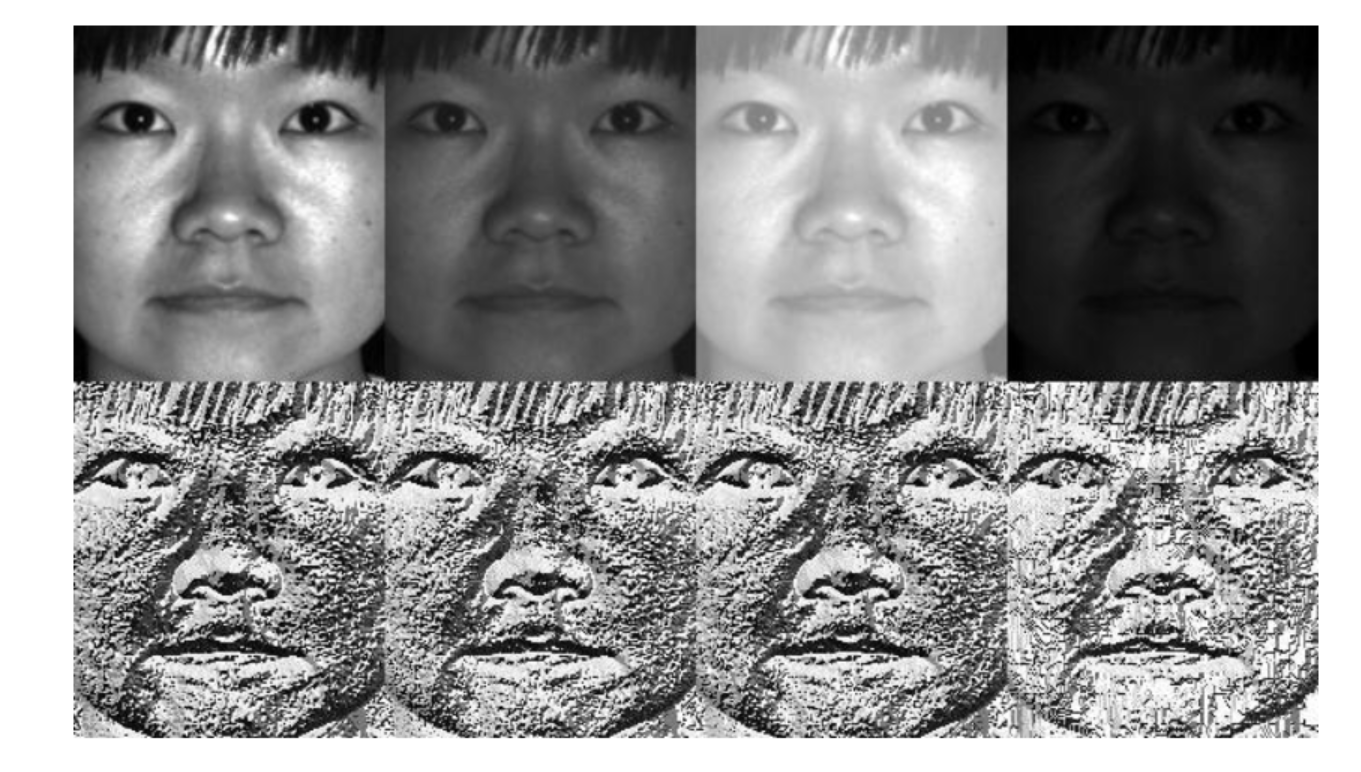
\includegraphics[width=0.7\linewidth]{grayscale.PNG}
\caption[De \emph{grayscale} para LBP
]{Imagens resultantes do algoritmo LBP abaixo, geradas à partir da imagem em \emph{grayscale} acima.}
\label{fig:graficosVariandoTamanhoRede}
\end{figure}
% é o proposto por Paul Viola e Michael Jones no 
% artigo  "Rapid Object Detection using a Boosted Cascade of Simple Features" em 2001. É uma abordagem
% baseada em Machine Learning em que uma função \emph{cascade} é treinada com o uso de muitas imagens
% positivas e negativas.


\section{Tecnologia de Hardware}

Todos os algoritmos que irão processar a imagem da câmera e aplicação do back end precisam ficar alocados num servidor. Assim sendo, foi
escolhido um raspberry pi zero W 1.1 para ser usado como o dispositivo que funcionará como servidor. Além disso, o Camera Module V2
será responsável por captar a imagem. Se fizermos uma comparação com os dispositivos de monitoramento presentes no mercado,
esses dispositivos não são muito potentes. A empresa força tarefa de Uberlândia que fornece serviços de segurança e portaria remota, por exemplo,
utiliza câmeras IP da Intelbras, muitas delas com sensores de visibilidade noturna, como o modelo VIP 3230 B SL. Por meio de uma conexão de rede, a informação de vídeo
dessas câmeras vai para os servidores da empresa que possuem alta capacidade de processamento. Entretanto, mesmo com a capacidade reduzida
dos dispositivos que serão usados neste trabalho, os algoritmos de reconhecimento facial, a aplicação do servidor e o front end poderão ser transferidos
para outros melhores.

% raspberry pi zero W V 1.1




\chapter{Revisão Bibliográfica}
%TCC:
Um ou mais capítulos (por exemplo, se há duas linhas de trabalhos relacionados).



\chapter{Desenvolvimento}
%TCC:
Um ou mais capítulos (por exemplo um para testes)


\begin{figure}[!ht]
    \centering
	
\includegraphics[width=0.55\linewidth]{imagemExemplo.pdf}
	\caption[Isso é o que aparece no sumário]{Imagem de exemplo.}
	\label{fig:graficosVariandoTamanhoRede}
\end{figure}


%TCC:
%TCC:
%TCC:
%TCC:

% ---
% Conclusão
% ---
\chapter[Conclusão]{Conclusão}
%TCC:
E daí?





% ----------------------------------------------------------
% ELEMENTOS PÓS-TEXTUAIS
% ----------------------------------------------------------
\postextual


% ----------------------------------------------------------
% Referências bibliográficas
% ----------------------------------------------------------
\bibliography{abntex2-modelo-references}


%% ----------------------------------------------------------
%% Apêndices TCC: só mantenha se for pertinente.
%% ----------------------------------------------------------

% ---
% Inicia os apêndices
% ---
\begin{apendicesenv}

% Imprime uma página indicando o início dos apêndices
\partapendices

% ----------------------------------------------------------
\chapter{Quisque libero justo}
% ----------------------------------------------------------

\lipsum[50]

% ----------------------------------------------------------
\chapter{Coisas que fiz e que achei interessante mas não tanto para entrar no corpo do texto}
% ----------------------------------------------------------
\lipsum[55-57]

\end{apendicesenv}
% ---


% ----------------------------------------------------------
% Anexos %TCC: so mantenha se pertinente.
% ----------------------------------------------------------

% ---
% Inicia os anexos
% ---
\begin{anexosenv}

% Imprime uma página indicando o início dos anexos
\partanexos

% ---
\chapter{Eu sempre quis aprender latim}
% ---
\lipsum[30]

% ---
\chapter{Coisas que eu não fiz mas que achei interessante o suficiente para colocar aqui}
% ---

\lipsum[31]

% ---
\chapter{Fusce facilisis lacinia dui}
% ---

\lipsum[32]

\end{anexosenv}

%---------------------------------------------------------------------
% INDICE REMISSIVO
%---------------------------------------------------------------------

\printindex



\end{document}